\section{Transformer}\label{model:Transformer}

\begin{multicols}{2} 
    \begin{figurehere}
    \centering
    
    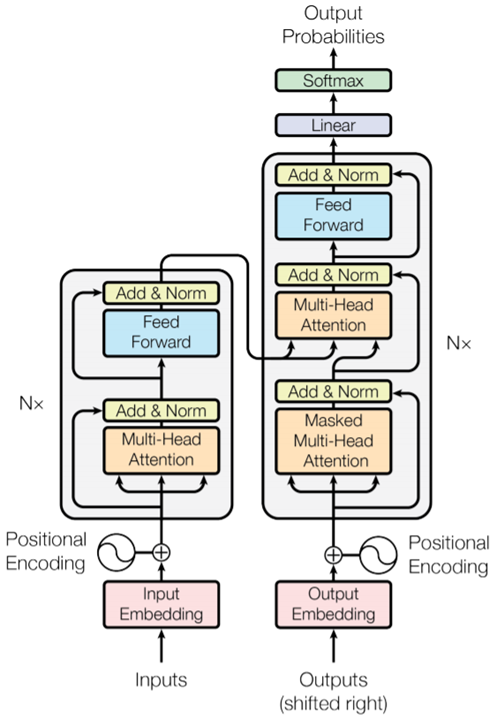
\includegraphics[width=9cm]{Encoder-Decoder/Transformer/Images/Trm Architecture.jpg}
    \caption{Transformer模型架构}
    \label{Trm:architecture}
\end{figurehere}
    %\noindent \textbf{Encoder}
    
    \begin{itemize}
        \justifying
        \item Input Embedding: 输入的token sequence embedding
        
        \item Positional Encoding位置编码满足下列特性
        1) 每个位置有唯一的位置编码
        \begin{align}
            PE(pos,2i)&=sin(\frac{pos}{1000^\frac{2i}{d_{model}}})\\
            PE(pos,2i+1)&=cos(\frac{pos}{1000^\frac{2i}{d_{model}}})
        \end{align}
        2) 由三角函数加法公式可求得相对距离$|pos_1-pos_2|$, 但\textcolor{red}{无法确定两个位置谁处于前面}
        \begin{equation}
            \begin{split}
                cos((pos_1-pos_2)*i)=cos(pos_1*i)cos(pos_2*i)\\
                +sin(pos_1*i)sin(pos_2*i)
            \end{split}
        \end{equation}
        
        \item Multi-Head Attention, 多头注意力模型
            \begin{enumerate}
                \item $Q_t=XW_Q, K_t=YW_K, V_t=ZW_V$; 一般Y, Z相同, 若X也相同则称为自注意力, <bs, seq, d>
                \item $Q_t$.reshape(bs, n, seq, d/n), $K_t$.reshape(bs, n, seq, d/n), $V_t$.reshape(bs, n, seq, d/n); n=\#heads
                \item Attention($Q_t$,$K_t$,$V_t$)=softmax($\frac{Q_tK_t^T + mask}{\sqrt{\textcolor{red}{d_k}}})V_t$; softmax用于归一化权重, 分母用于归一化协方差, mask矩阵中负无穷元素值表示masked token或pad; 
                \item Attention.reshape(bs, seq, d) 
            \end{enumerate}
        
        \item FNN前向回馈网络: $activate(xW_1+b_1)W_2+b_2$
        \begin{itemize}
            \item [$\triangleright$] $W_1$, $<d, d_{ff}>$
            \item [$\triangleright$] $W_2$, $<d_{ff}, d>$
        \end{itemize}
         
        \item Output Embedding: 同语种时与Input Embedding一致, 不同语种时(如处理翻译任务)则是另一Learnable Embedding
    \end{itemize}
    %\noindent Decoder
    %\begin{itemize}
    %    \item ss
    %\end{itemize}
\end{multicols}
